\section{Termination Proof of \texttt{TACo}} \label{sec:proof}

The proof of \texttt{TACo}'s termination (with an agreement) involves three steps. First, we show that \texttt{TACo} always enters a cycle, where the auction steps repeat in a loop as defined in \Cref{def:cycle}. Next, we demonstrate that profit differences between choices within a cycle are bounded, with the bound proportional to the trading unit per step $d$. This restricts each agent’s available choices to options with profit differences no greater than the bound. Finally, we prove that \texttt{TACo} satisfies the epsilon-termination condition and hence converges. 

The intuition behind the convergence of \texttt{TACo} lies in that, as soon as a cycle is detected, the trading unit $d$ is reduced by a fixed decrement factor $\decFactor$. However, as $d$ decreases, the profit differences within the cycle shrink and must thus eventually fall below the threshold $\epsilon$ for all agents. At this point, the agents reach a consensus by definition, and \texttt{TACo} terminates.

\begin{figure}[hbt!]
    \centering
\hspace*{-0.01\textwidth}
\resizebox{0.5\textwidth}{!}{
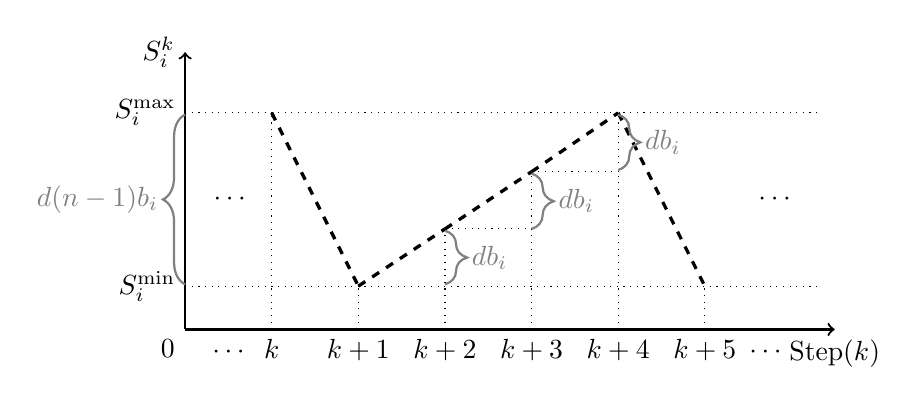
\begin{tikzpicture}[thick, scale=1.1][hbt!]
    % Axes
    \draw[->] (0,0) -- (7.5,0) node[below] {Step$(k)$};
    \draw[->] (0,0) -- (0,3.2) node[left] {$S_i^k$};

    % Horizontal dashed lines
    \draw[thin, dotted] (0,2.5) -- (7.3,2.5) node[anchor=east] at (0,2.5) {$S_i^{\max}$};
    \draw[thin, dotted] (0,0.5) -- (7.3,0.5) node[anchor=east] at (0,0.5) {$S_i^{\min}$};
    \draw[thin, dotted] (3,0.5+0.66) -- (4,0.5+0.66);
    \draw[thin, dotted] (4,0.5+0.66*2) -- (5,0.5+0.66*2);

    % Labels
    \node[below left] at (0,0) {$0$};
    \node[below] at (1,0) {$k$};
    \node[below] at (2,0) {$k+1$};
    \node[below] at (3,0) {$k+2$};
    \node[below] at (4,0) {$k+3$};
    \node[below] at (5,0) {$k+4$};
    \node[below] at (6,0) {$k+5$};
    \node[below] at (6.7,-0.07) {$\cdots$};
    \node[below] at (0.5,-0.07) {$\cdots$};

    % Dotted vertical lines for steps
    \draw[thin, dotted] (1,0) -- (1,2.5);
    \draw[thin, dotted] (2,0) -- (2,0.5);
    \draw[thin, dotted] (3,0) -- (3,0.5+0.66);
    \draw[thin, dotted] (4,0) -- (4,0.5+0.66*2);
    \draw[thin, dotted] (5,0) -- (5,2.5);
    \draw[thin, dotted] (6,0) -- (6,0.5);

    % Connecting dashed lines
    \draw[very thick, dashed] (1,2.5) -- (2,0.5);
    \draw[very thick, dashed] (2,0.5) -- (3,0.5+0.66);
    \draw[very thick, dashed] (3,0.5+0.66) -- (4,0.5+0.66*2);
    \draw[very thick, dashed] (4,0.5+0.66*2) -- (5,2.5);
    \draw[very thick, dashed] (5,2.5) -- (6,0.5);
    \node[right] at (6.5,1.5) {$\cdots$};
    \node[left] at (0.82,1.5) {$\cdots$};
    
    % Bracket
    \draw[decorate, decoration={brace, mirror, amplitude=8pt}, gray] 
        (0,2.48) -- (0,0.52) node[midway, left=6pt, gray] {$\textstyle d(n-1)b_i$};
    \draw[decorate, decoration={brace, mirror, amplitude=8pt}, gray]
        (3,0.52) -- (3,0.5+0.64) node[midway, right=6pt, gray] {$\textstyle db_i$};
    \draw[decorate, decoration={brace, mirror, amplitude=8pt}, gray]
        (4,0.5+0.66) -- (4,0.5+0.66*2-0.02) node[midway, right=6pt, gray] {$\textstyle db_i$};
    \draw[decorate, decoration={brace, mirror, amplitude=8pt}, gray]
        (5,0.5+0.66*2+0.02) -- (5,2.48) node[midway, right=6pt, gray] {$\textstyle db_i$};
\end{tikzpicture}
}
\caption{(Illustration of \Cref{theorem:lemma1}, $n=4$) This figure states that the row sum $S_i^k$ of the $i$-th row of the profit matrix $\profitList$ remains constant every $n$ steps. The fluctuations in the row sum are bounded by the difference $S_i^{\text{max}} - S_i^{\text{min}} = d(n-1)b_i$, where $S_i^{\text{max}}$ and $S_i^{\text{min}}$ denote the maximum and minimum row sums during the cycle. The diagram highlights the periodic nature of the row sum across steps and the incremental fluctuations $db_i$ within each step.}
\label{fig:fluctuations}
\end{figure}

\subsection{Existence of cycles in \texttt{TACo}}
We first prove that \texttt{TACo} always enters a cycle. A cycle occurs when the auction steps repeat in a loop, as defined in \Cref{def:cycle}. This result is established by analyzing bounded row sums and discrete profit increments. The following lemma shows that the row sum of the profit matrix fluctuates within a bounded range as shown in \Cref{fig:fluctuations}.

\begin{lemma}[Row sum of the profit matrix] \label{theorem:lemma1}
The row sum $S_i^k = \sum_{j=1}^m \profitList_{i,j}^k$, where $m$ is the number of choices, remains constant every $n$ steps, with fluctuations equal to:
\begin{equation}
    \smax - \smin = d(n-1)b_i,
\end{equation}
where $\smax$ and $\smin$ are the maximum and minimum row sums that can occur during the \texttt{TACo} process.
\end{lemma}

The bounded row sums imply that the actual profit values $\profitList_{ij}$ are lower bounded, as established in the next lemma.

\begin{lemma}[Lower bound of profit values] \label{theorem:lemma2}
The profit value $\profitList_{ij}$ for any agent $i$ and choice $j$ is lower bounded as
\begin{equation}
    \profitList_{ij} \geq \min\left(\min(\profitList_{i,:}^{0}), \textstyle{\frac{\smin}{m}} - d(n-1)b_i\right),
\end{equation}
where $m$ is the number of choices and  $\min(\profitList_{i,:}^{0})$ is the minimum element for row $i$ in the initial profit matrix $\profitList$.
\end{lemma}

Since the row sums of the profit matrix $\profitList$ remain constant over every $n$ steps (Lemma 1) and since $\profitList$ is lower-bounded (Lemma 2), it directly follows that  $\profitList$ is also upper-bounded. We state this consequence in the following corollary.


\begin{corollary}[Upper bound of profit values] \label{theorem:corollary1}
 The profit values in the matrix $\profitList$ are upper bounded.
\end{corollary}


Exploiting the proved upper and lower bounds on $\profitList$ derived so far, we can now formally prove that \texttt{TACo} always enters a cycle. This result is important because, by definition, a state of consensus where all agents have similar preferences -- up to a level of tolerance $\epsilon$ -- is also a cycle. Hence, the convergence of \texttt{TACo} will subsequently boil down to showing that the cycle it eventually falls into corresponds to a consensus.

\begin{theorem}[The auction always falls into a cycle] \label{theorem:theorem1}
Let $\mathcal{S}$ be the set of all possible agent-profit matrix tuples $(i, \profitList)$, where $i \in [n]$ and $\profitList$ is a profit matrix satisfying the constraints defined in 
\Cref{theorem:lemma1}, \Cref{theorem:lemma2} and \Cref{theorem:corollary1}. The \texttt{TACo} algorithm must eventually revisit a previously encountered tuple $(i, \profitList) \in \mathcal{S}$, resulting in the formation of a cycle.
\end{theorem}

\subsection{Bounded profit differences between choices in a cycle}

Having established that \texttt{TACo} always enters a cycle, we now focus on bounding the profit differences among the choices within that cycle. More importantly, we will show that the underlying bound in profit differences is \textit{proportional} to $d$; a property that will allow us to prove  \texttt{TACo} eventually converges to a state of agreement between agents, particularly since $d$ is decremented according to \eqref{eq:dr} once a cycle is detected.  To establish this property, we start by introducing the \textit{choice count matrix} (\(\Delta^\cycle\)), which tracks how many times each agent selects each choice during a cycle.

\begin{definition}[Choice count matrix, $\Delta^\cycle$] 
The choice count matrix, denoted as $\Delta^\cycle \in \mathbb{Z}_{\geq 0}^{n \times m}$, represents the number of times each choice is selected by agents during a cycle. Specifically, $\Delta^\cycle_{i,j}$ denotes the number of times agent $i$ selects choice $j$ within the cycle $\cycle$. 
\end{definition}

It follows that the matrix $\Delta^\cycle$ satisfies the following:
\begin{equation} \label{eq:choiceCountToPay}
    \payList^{t+\ell} - \payList^t = nd \cdot \Delta^\cycle,
\end{equation}
\begin{equation} \label{eq:choiceCountToOffer}
    \offerList^{t+\ell} - \offerList^t = d \cdot H_n \Delta^\cycle,
\end{equation}
where $\payList^{t+\ell} - \payList^t$ and $\offerList^{t+\ell} - \offerList^t$ represent the net changes in the pay matrix and offer matrix after each cycle of length $\ell$, respectively, and $H_n = \textbf{1}_n \textbf{1}_n^\top$ is an $n \times n$ matrix with all elements equal to 1, capturing the aggregation of offers received across all agents. Using the definition of the choice count matrix and its relationship shown in \cref{eq:choiceCountToPay} and \cref{eq:choiceCountToOffer}, we establish the structure of $\Delta^\cycle$ which shows that, within a cycle, all agents select each choice the same number of times.

\begin{lemma}[Uniform choice count matrix in a cycle] \label{theorem:lemma3}
The choice count matrix $\Delta^\cycle \in \mathbb{Z}_{\geq 0}^{n \times m}$ for a cycle  has the form
\begin{equation}
\Delta^\cycle = \begin{bmatrix}
    c_1 & c_2 & \ldots & c_m \\ 
    \vdots & \vdots & \ddots & \vdots \\ 
    c_1 & c_2 & \ldots & c_m 
\end{bmatrix},
\end{equation}
where each $ c_j \in \mathbb{Z}_{\geq 0} $ represents the number of times that choice $ j $ is selected by each agent within the cycle.
\end{lemma}

This uniform structure naturally leads to the concept of \emph{active choices}: the choices selected by agents during a cycle.

\begin{definition}[Active choices in a cycle, $A^\cycle$] The active choices in a cycle, denoted $A^\cycle$, are the row indices of the choice count matrix $\Delta^\cycle$ with non-zero values.  In other words, $A^\cycle$ is a set of indices representing the choices selected at least once by some agent within a cycle.
\end{definition}

We now analyze the profit differences within a cycle by focusing on active choices only. Leveraging \Cref{theorem:lemma1}, \Cref{theorem:lemma2}, and \Cref{theorem:lemma3}, we prove a key result that bounds these profit differences \textit{proportionally} to the amount of trading units $d$.

\begin{theorem}[Bound on profit differences within a cycle] \label{theorem:theorem2}
The profit difference among the active choices $A^\cycle$ in a cycle $\cycle$ for agent $i$ is bounded as 
\begin{equation} \label{eq:profDiff_Theorem2}
U_\cycle^i - L_\cycle^i \leq (m+1)d(n-1)b_{\max},\quad \forall i \in [n],
\end{equation}
where $m$ is the total number of choices, $d$ is the trading unit for the current cycle, $b_{\max} = \max_{i \in [n]} (b_i)$ is the highest private valuation among the agents, and $U_\cycle^i$ and $L_\cycle^i$ are the maximum and minimum profit values for the active choices of agent $i$ within cycle $\cycle$, respectively.
\end{theorem}

\subsection{Finite termination property of \texttt{TACo}}
With the profit differences bounded proportionally to $d$ (\Cref{theorem:theorem2}), we now demonstrate that \texttt{TACo} satisfies the epsilon-termination condition, leading to an approximate agreement in a finite number of steps. Recall that each time a cycle is detected -- which provably happens according to Theorem \ref{theorem:theorem1} -- the algorithm reduces the trading unit $d$ by a fixed decrement factor $\decFactor$. This reduction ensures that the profit differences between choices eventually fall below the threshold $\epsilon$, leading to termination.

\begin{theorem}[Termination of \texttt{TACo}] \label{theorem:theorem3}
The \texttt{TACo} algorithm terminates in a finite number of steps.
\end{theorem}

We also provide a practical bound on the worst-case number of steps required till termination. This bound accounts for the number of cycles needed to meet the epsilon-termination condition as well as the steps within each cycle, hence providing practical insights into the efficiency of \texttt{TACo}.

\begin{theorem}[Termination bound for \texttt{TACo}] \label{theorem:theorem4}
    The \texttt{TACo} algorithm terminates at most within the following number of steps:
    \begin{equation} \label{eq:terminationBound}
        \textstyle{
        \left\lceil \log_{\decFactor} \left(\frac{\epsilon}{(m+1)d_0(n-1)b_{\max}} \right) \right\rceil \cdot n \cdot \big((m+1)(n-1)\big)^{nm}},
    \end{equation}
    with decrement factor $\decFactor$ and initial trading unit $d_0$.
\end{theorem}

\Cref{theorem:theorem4} implies that if $\epsilon$ is increased to $\frac{\epsilon}{\decFactor}$, then the worst-case termination bound decreases by $n \cdot \big((m+1)(n-1)\big)^{nm}$ steps. 